\documentclass[12pt,a4paper]{article}
\usepackage[utf8]{inputenc}
\usepackage[T1]{fontenc}
\usepackage[french]{babel}
\usepackage{setspace}
\usepackage{geometry}
\usepackage{graphicx}
\usepackage{array}
\usepackage{parskip}

%%%

\usepackage{fancyhdr}
\pagestyle{fancy}

% En-tête (logo INSA en haut à gauche)
\fancyhead[L]{
\includegraphics[height=1.5cm]{INSA_logo.png}}

% Pied de page (logo graphique rouge en bas à droite)
\fancyfoot[R]{
\includegraphics[height=1.5cm]{INSA_graphic.png}}

% Supprimer le numéro de page automatique si besoin
\fancyfoot[C]{}
\renewcommand{\headrulewidth}{0pt}
\renewcommand{\footrulewidth}{0pt}

%%%

\geometry{margin=2.5cm}

\begin{document}

\begin{center}
    \Large \textbf{CONVENTION DE PRÊT D'ORDINATEURS PORTABLES}
\end{center}

\vspace{1cm}

Entre \\
\textbf{L’Institut National des Sciences Appliquées de Rennes},\\
Établissement public à caractère scientifique, culturel et professionnel, \\
20 avenue des Buttes de Coësmes -- CS 70839 - 35708 RENNES Cedex 7 \\

Agissant tant en son nom que pour le compte du département Informatique (INFO) de l’INSA Rennes, \\

Représenté par Monsieur Vincent BRUNIE en sa qualité de Directeur \\

Ci-après désignée « l’INSA » \\

\textbf{Et} \\

Madame / Monsieur \textbf{ {{ nom }} {{ prenom }} } \\
Inscrit(e) en (intitulé du diplôme) Spécialité Informatique \\
Année d’étude : {{ annee_etude }} \\
N° INE : {{ ine }} \\

Désigné ci-dessous « le bénéficiaire ». \\

\rule{\linewidth}{1pt} \\

Il est convenu ce qui suit :

\section*{Article 1\textsuperscript{er} : Objet}

\subsection*{1.1}
Le prêt d'ordinateurs portables est réservé aux étudiants inscrits au département INFO.  
L'attribution du matériel est décidée par une commission du département INFO composée du directeur du département et des 3 responsables d'années.

\subsection*{1.2}
Lors d’un prêt, le bénéficiaire doit fournir les pièces suivantes :
\begin{itemize}
    \item la convention de prêt d'ordinateurs portables, datée et signée,
    \item un chèque de caution de 110€ ou un virement bancaire auprès de l’agence comptable de l’INSA Rennes, à l’exception des étudiants boursiers.
\end{itemize}

Si le virement bancaire est choisi, indiquer sur le libellé du virement « PCINFO Nom Prénom ».\\

\textbf{RIB de l’INSA ci-dessous :}

\begin{center}
\fbox{
    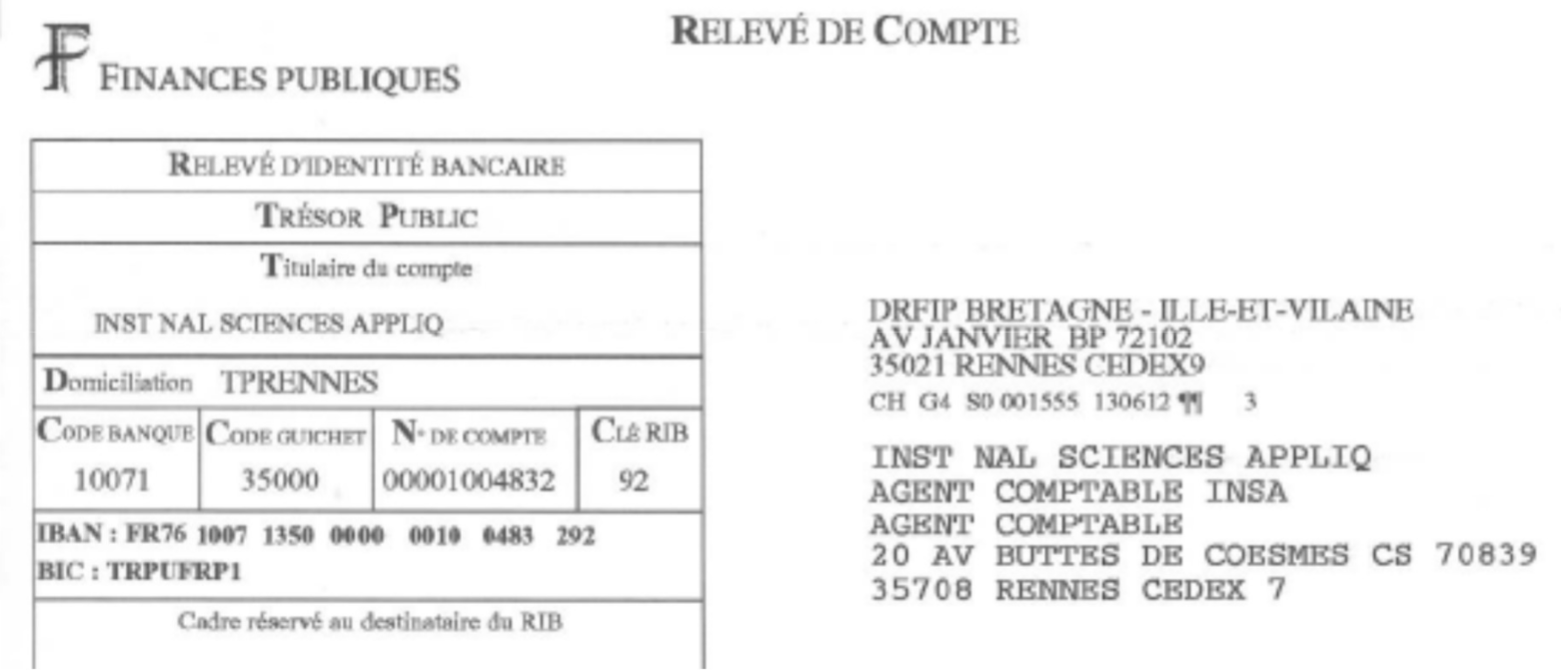
\includegraphics[width=0.9\linewidth]{INSA_RIB.png}
}
\end{center}

%----------------------------------------------
\section*{Article 2 : Description du matériel}

\subsection*{2.1}
Le bénéficiaire déclare avoir reçu en main propre : \\
Description du matériel, description technique, dont accessoires :
\begin{itemize}
    \item Désignation matériel : «Désignation\_matériel»
    \item Numéro d’inventaire : «N\_INVENTAIRE»
    \item Numéro de série : «N\_SERIE»
\end{itemize}

%----------------------------------------------
\section*{Article 3 : Durée du prêt}

Le département INFO prête le matériel décrit ci-dessus pour une période de :

\begin{center}
\begin{tabular}{|l|l|}
\hline
\textbf{Année} & \textbf{Durée maximale} \\
\hline
Étudiants en 3\textsuperscript{e} année INFO & Jusqu’à 3 ans, soit juin 2027 \\
Étudiants en 4\textsuperscript{e} année INFO & Jusqu’à 2 ans, soit juin 2026 \\
Étudiants en 5\textsuperscript{e} année INFO & Jusqu’à 1 an, soit juin 2025 \\
\hline
\end{tabular}
\end{center}

Lorsque l’étudiant n’est plus inscrit au département informatique de l’INSA, il devra restituer le matériel emprunté même si la période consentie n’est pas terminée.  
Le bénéficiaire s’engage à rendre le matériel à une date définie par le département INFO et au plus tard lorsqu’il n’est plus inscrit à l’INSA.

%----------------------------------------------
\section*{Article 4 : Conditions du prêt}

4.1 Le prêt et le retour s’effectuent au département informatique selon les créneaux définis.

\medskip
4.2 Le bénéficiaire du matériel versera un chèque de caution d’un montant de 110€ qui sera encaissé ou un virement bancaire confirmé par l’agence comptable en échange de la remise du matériel (sauf étudiants boursiers). Le montant lui sera restitué lorsqu’il rendra le matériel.

\medskip
4.3 Le prêt consenti ne donne pas lieu à paiement d’une redevance à l’établissement pendant la période d’application de la présente convention.

\medskip
4.4 L’INSA et plus précisément le département INFO ne peuvent être tenus pour responsables en cas d’utilisation frauduleuse ou illicite du matériel emprunté. À ce titre, l’utilisateur est tenu de respecter les règles et usages en vigueur dans l’établissement.

\medskip
4.5 En cas de dysfonctionnement, le matériel devra être immédiatement remis au département INFO.  
Le dysfonctionnement sera précisément signalé par l’emprunteur et mentionné sur la Convention de prêt.  
Le département INFO ne sera pas tenu responsable d’une perte des données personnelles.

\medskip
4.6 Le département INFO ne prend pas en charge les installations logicielles du matériel.

\medskip
4.7 À l’issue de la période de prêt, le matériel est rendu et toutes les données personnelles sont effacées.  
Il appartient au bénéficiaire de sauvegarder ses données.

%----------------------------------------------
\section*{Article 5 : Détérioration, perte et vol}

5.1 En cas de détérioration, perte ou vol du matériel, l’étudiant indemnisera l’INSA. À lui de se tourner vers son assureur.

\medskip
5.2 En cas de perte ou de vol, l’emprunteur avertit immédiatement l’établissement et fournit les déclarations attestant l’événement.  
En cas de vol, il doit faire un dépôt de plainte et en transmettre une copie.  

Le remboursement est à la charge de l’emprunteur :
\begin{itemize}
    \item matériel acheté dans l’année : remboursement de la valeur d’achat TTC
    \item matériel plus ancien : remboursement de la valeur vénale
\end{itemize}

\medskip
5.3 En cas de détérioration :
\begin{itemize}
    \item si irréparable : indemnisation selon 5.2
    \item si réparable : indemnisation du coût de la réparation
\end{itemize}

%----------------------------------------------
\section*{Article 6 : Restitution hors délai}

6.1 En cas de non restitution, suspension de prêt égale au nombre de jours de retard.  
Une redevance de 10\% de la valeur d’achat du matériel par mois entamé peut être exigée (dans la limite de la valeur d’achat).

\medskip
6.2 En cas de retard pour raison médicale, un justificatif doit être fourni. La commission décide de l’application ou non de la redevance.

%----------------------------------------------
\section*{Article 7 : Sanctions}

En cas de non-paiement, l’INSA pourra exclure le bénéficiaire du service de prêt et saisir la section disciplinaire.

\vspace{0.5cm}
\rule{\linewidth}{1pt}
\vspace{0.5cm}

Fait en un exemplaire original, à Rennes, le : {{ date }}.

\vspace{0.5cm}

\textbf{Le bénéficiaire (« Lu et approuvé »)} 

\vspace{0.4cm}

Observations lors de l’emprunt : {{ obs }}

\vspace{0.4cm}

Signature :

\vspace{0.3cm}

\begin{minipage}{0.5\linewidth} 
\end{minipage} 
\hfill 
\begin{minipage}{0.5\linewidth} 
\textbf{Pour le département INFO :} \\[0.3cm] 
Atteste du prêt du matériel \\[0.4cm] 
\begin{center} 
\textbf{Le directeur de l’INSA} \\ 
\end{center} 
\end{minipage}

\vspace{1.2cm}

Retour du matériel effectué le : \underline{\hspace{2cm}}/\underline{\hspace{2cm}}/\underline{\hspace{2cm}}

\vspace{0.5cm}

État du matériel lors du retour : \\

\vspace{0.25cm}

Remarques : \\

\vspace{0.4cm}

Signature de l’emprunteur :
\end{document}
